\chapter{Towards Scene-Aware Acoustic Rendering Pipelines for Augmented Audio Reality}\label{ch:ar-pipeline}% If you're changing this, update Section 1.6
The following Chapter details the implementation to address the primary objective of the thesis.

\section{Overview}\label{sec:overview}
The proposed system aims to produce realistic sound transmissions between sound-emitting holograms in AR space and a listener who is experiencing the holograms via a head-mounted holographic display and perceived auditory stimuli via headphones. In this chapter, the term ``listener'' is used interchangeably with the term ``user'' to refer to the user who is displayed audio-visual stimuli from both the holographic HMD and the headphones. The implementation of this method for interactive sound rendering is demonstrated on a Microsoft Hololens 2 Augmented Reality Head-Mounted Headset, an embedded wearable computer with a holographic display featuring space-sensing and spatial mapping technology that enables Simultaneous Localisation and Mapping (SLAM) methods \cite{davison2003real, ungureanu2020hololens}.

\begin{figure}[htb]
    \centering
    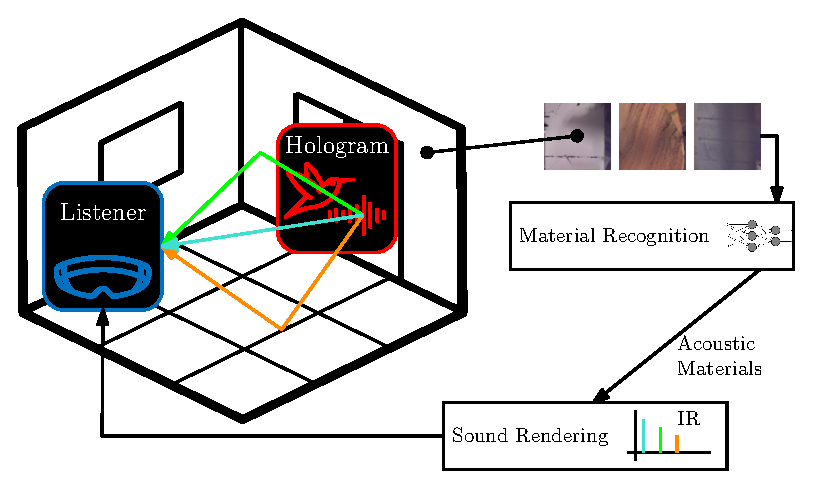
\includegraphics[width=1\linewidth]{ar-system}
    \caption{Overview of the presented method: an Augmented Reality user and listener, the blue icon, is perceiving audio-visual stimuli through headphones and a head-mounted display, experiencing virtual holograms projected onto his surroundings. The proposed system aims at the realistic rendering of sound transmissions from sound-emitting holograms and the listener.}
\label{fig:method-overview}
\end{figure}

\section{Dynamic Environment Reconstruction}
The first chain in the process of generating realistic sound transmission between a listener and holograms in AR space is the generation and handling of a virtual environment to host scene elements such as virtual sound-emitting entities. In AR space, the scene geometry includes a reconstruction of the real space surrounding the user. The space surrounding the user is sensed using space-sensing technology featured in the Hololens 2 device \cite{ungureanu2020hololens}. Using the Microsoft Mixed Reality Toolkit~\footnote{https://github.com/microsoft/MixedRealityToolkit-Unity}, an environment mesh is continuously extracted as a triangulated mesh and updated every 3 to 5 seconds, reflecting dynamic changes in the environment like furniture being moved or a crowd entering the space.\par
The triangulated mesh, represented as a list of triangles and indices, is used to construct a Bounding Volume Hierarchy (BVH), where triangle primitives are wrapped in Axis-Aligned Bounding Boxes (AABBs), optimising geometrical search operations for acoustic modelling such as ray-triangle intersection tests. As discussed in Section~\ref{sec:bg-geometry-handling}, One key advantage of using a BVH in the pipeline is the ability to group multiple primitives in AABBs whose size can be determined by a geometry reduction algorithm to simplify the environment complexity whilst maintaining a target perceptual response from the acoustic model. \par
\begin{figure}[htb]
    \centering
    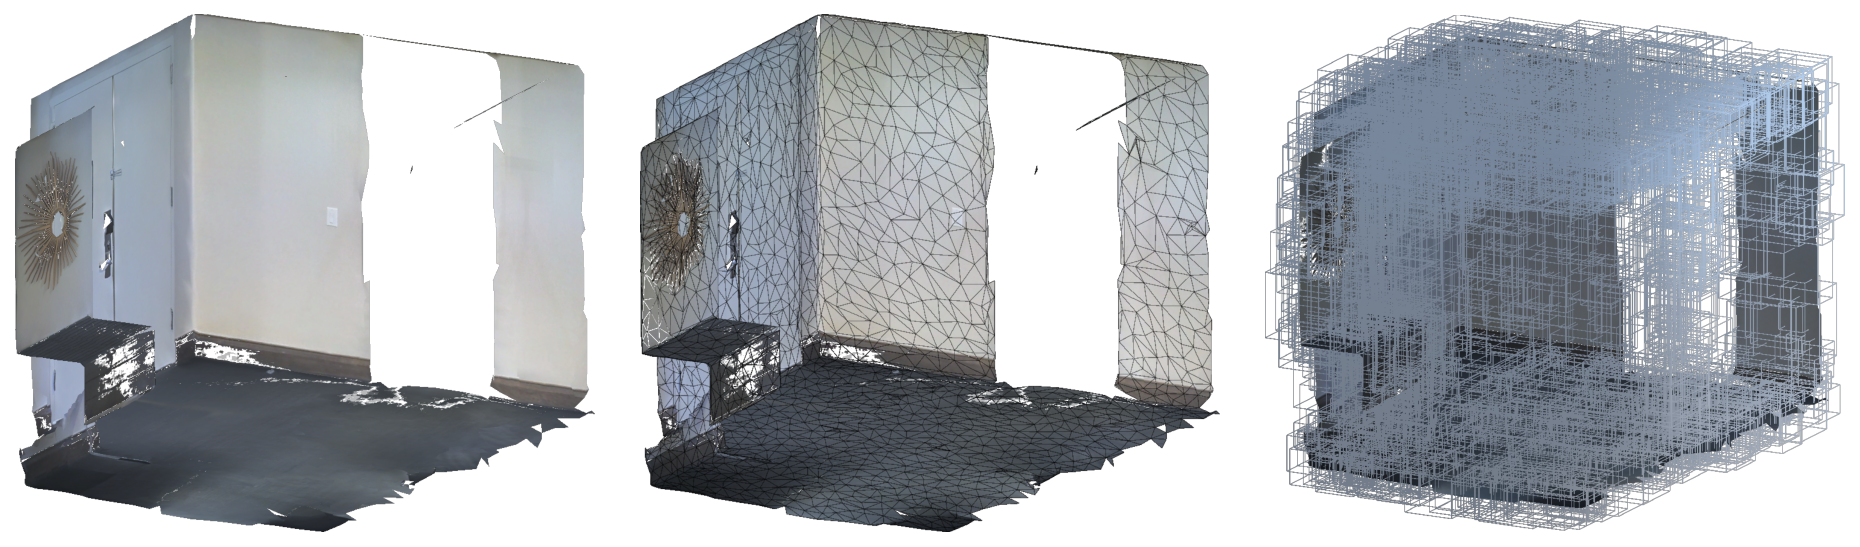
\includegraphics[width=1\linewidth]{bvh-matterport}
    \caption{A visualisation of a BVH constructed on a portion of a scanned environment, left image, to demonstrate how AABBs encapsulate triangle primitives, visible in the centre image, forming a tree of boxes to partition the geometry.}
\label{fig:bvh-visualisation}
\end{figure}
The BVH implementation supports traversing and optimisation operations, allowing the BVH tree representing the environment to support deformation and moving objects at interactive rates \cite{wald2007ray}.

\section{Material Tagging from Partitioned Space}
One key advantage of the employment of AABBs-based BVH for the handling of scene geometry is the space partitioning that can be used for the material tagging process. As discussed in Chapter~\ref{ch:Materials}, CNNs offer efficient approaches to mapping the appearance of surfaces to the acoustic characteristics of their materials, like absorption or scattering coefficients. The space partitioning provided by the BVH here is used to capture the appearance of portions of the reconstructed environment in order to determine the material characteristics of its surfaces.\par

\section{Acoustic Rendering Pipeline}

\subsection{Overview}
The geometry handling system provides the foundations for supporting real-time auralisations in AR, as it provides a solution to the problem of defining acoustic geometry: auralisations can be produced from simplistic cuboid volume to realistic reconstructions of space with orders of fidelity to the physical counterparts of millimetres. Computational costs associated with generating auralisations often rise with the number of geometrical primitives used in the reconstructed space: in triangulated meshes, detailing smaller structures in a 3D model increases the number of triangles. Detailed scene geometry allows approximation of acoustic phenomena and generally contributes to high-resolution soundfield modelling, though the computational requirements make it unfeasible for interactive applications. As discussed in Chapter~\ref{ch:litReview}~and~\ref{ch:acousticrendering}, studies outline a perceptual threshold and benchmark to define the minimum level of detail required from reconstructions, and recent research on acoustic simulations conducted over the last decades has expanded towards defining what is required from a virtual environment to produce a believable simulation. Combined with advances in real-space scanning technology and user-friendly 3D reconstruction software, it is now possible to create appropriate virtual environments for acoustic simulations without requiring expert computer graphics engineering knowledge.\par

\subsection{Selecting Acoustic Rendering Techniques}
A central problem inherent in the task of interactive soundfield approximations for generating dynamic auralisations is the task of adopting a method for propagating anechoic audio in a dynamic scene. As discussed in Chapter~\ref{ch:Background} there are families of sound rendering techniques that produce auralisations with varying levels of realism evoked by audio propagated in the simulated soundscape and associated computational costs, as well as limitations due to their inherent architecture or nature.

Ray-based techniques, wave-ray hybrid techniques, and wave-based techniques have emerged as prominent methods to generate impulse responses in the field of acoustics, each contributing to understanding how sound propagates within a given space. Ray-based techniques, rooted in geometric acoustics, simulate sound by tracing rays that emanate from a source and bounce off various surfaces within a space. This method creates echoes and reverberations, contributing to the overall impulse response. Notably, it offers efficiency as it's computationally less demanding compared to wave-based techniques, making it suitable for real-time applications or large-scale spaces often found in cultural heritage contexts. The geometrical nature of ray-based methods allows for easier integration with existing architectural models or historical reconstructions, and the method's inherent flexibility makes it easily adjustable to different acoustic scenarios. IS THIS OK FOR DYNAMIC AURALISATIONS

On the other hand, wave-ray hybrid techniques present a more complex picture, combining aspects of ray-based and wave-based methods. Rays are utilised to model the high-frequency components of the sound, while wave equations handle the low-frequency behaviour, attempting to capture the best attributes of both methods. However, the hybrid nature often means more computational resources are needed, and it might not always be the most suitable choice for cultural heritage applications where both high and low-frequency accuracy is not often the primary concern. IS THIS OK?

Wave-based techniques stand out for their precision, solving the wave equation to simulate how sound waves propagate through a space, accurately modelling diffraction, scattering, and other complex wave phenomena. While highly accurate, wave-based techniques often require substantial computational resources, making them less suited for real-time or large-scale applications. Moreover, this level of detail may exceed what is necessary for conveying the historical or cultural experience.

Considering the landscape of immersive acoustics, ray-based techniques offer a compelling option for cultural heritage contexts. Their computational efficiency, relative simplicity, and adaptability in handling various scenarios effectively capture the essential acoustic characteristics of historical spaces. Unlike wave-based or hybrid methods, ray-based techniques can prioritise the aspects most relevant to the experience and understanding of cultural heritage, aligning well with the objectives and constraints often found in this field. Therefore, while the high accuracy of wave-based methods or the comprehensive nature of hybrid methods may have specific applications in areas of cultural heritage investigations, it is the ray-based techniques (such as those employed by acoustic simulation software such as ODEON) that generally stand out as the most appropriate choice for the unique challenges and opportunities presented within the context of cultural heritage.

\subsection{Real-Time Spatial Audio Rendering Techniques}

So far the proposed system approximates acoustic phenomena from a dynamic environment reconstructed as the user interacts and navigate the complex scene, considering physical and objective factors of the soundscape. The HAS, however, is the final and crucial link in the chain of the reproduction system, requiring the pipeline to consider psychoacoustic and human factors in the generation of auditory stimuli expressed as binaural audio. The integration of factors of the HAS and the convolution of anechoic audio completes the 3D spatial audio chain.\par
Head-Related Impulse Responses (HRIRs) offer a compact solution to the integration of HAS features, much like room responses, as we can convolve a monaural signal to the frequency representation of a pair of HRIRs (one for each ear), the Head-Related Transfer Function (HRTFs). Hence, the discussed real-time convolution algorithms [REF] can be used, in combination with the $h$ RIR signal, to generate binaural rendered audio channels $y_{left}$ and $y_{right}$ from a monaural signal $x$:
\begin{equation}
    y_{left} = x * HRTF_{left} * h \quad \textrm{and} \quad  y_{right} = x * HRTF_{right} * h \textrm{.}
\end{equation}
HRTF channels left and right are evaluated in real-time, depending on the current position and rotation of the listener entity in the virtual environment, using a loaded bank or HRIRs that are often real measurements of subjects across a grid of points in the azimuth and elevation surrounding the subject. These measurements record the response of each ear canal, from a source position in the surrounding sphere, allowing an interactive HRIR algorithm to interpolate between these measurements. A range of objective metrics are commonly used in acoustic measurements. These metrics together offer a holistic understanding of acoustic properties of spaces, such as reverberation, clarity, strength, directionality, and intelligibility, and can be applied in various contexts, from concert halls to cultural heritage sites. 


\section{Implementation of an AR Prototype System for AAR}

\subsection{Overview}
The system uses a common game engine.
\begin{figure}[htb]
    \centering
    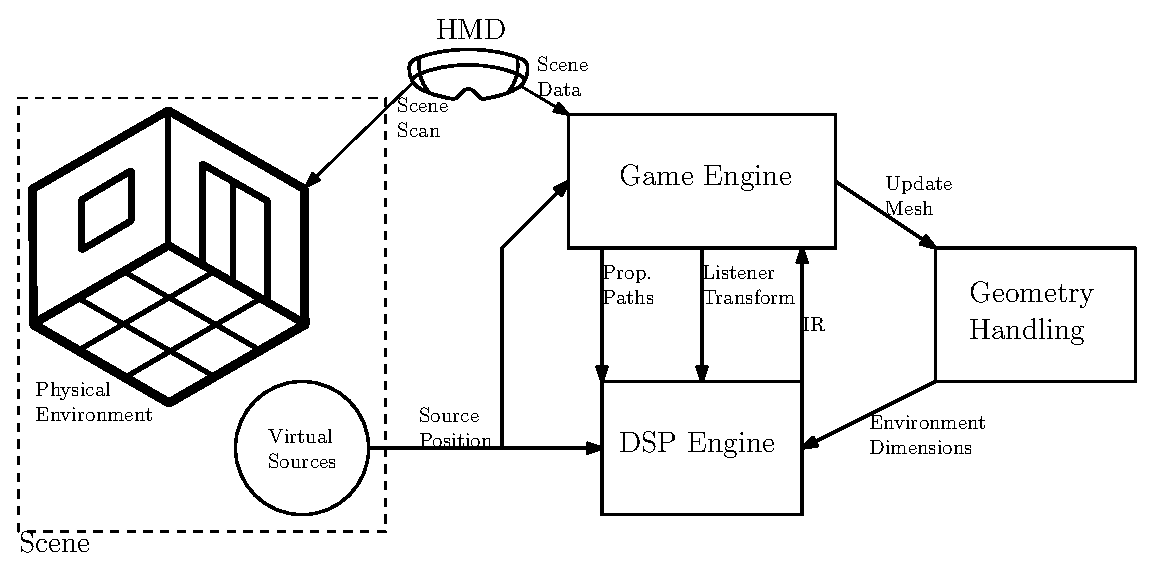
\includegraphics[width=1\linewidth]{ar-pipeline-diagram}
    \caption{An overview of the technical implementation of the proposed pipeline for spatial audio rendering applied to an Augmented Reality interactive application. }
    \label{fig:ar-pipeline-overview}
\end{figure}

\subsection{Hardware Apparatus}
Hololens 2

\subsection{Game Engine and Scene Management System}
Sound sources in AR scene.

\subsection{API Design for Spatial Audio Rendering}
DSPToolbox

\subsection{Acoustic Geometry Handling in Real-Time}
Async rendering or server-side rendering approaches

\subsection{Extension to multiple sources and source clustering}
Future work.


\section{Vision for Dynamic Auralisation Systems}
This section outlines the design of future prototypes for dynamic auralisations expanding from the proposed systems towards real-time interpolation 

\subsection{Using Radiance Fields for Inferring Local Acoustic Features of Reconstructed Space}

BVH space handling with image2reverb projections
local feature query via neural radiance field

